\documentclass{article}
\usepackage[utf8]{inputenc}
\usepackage{graphicx,amsmath,amsfonts,amssymb,caption,subcaption}

\begin{document}
\title{SVVR Assignment 2}
\author{Sander Nugteren (6042023) \and Merel de Groot (6103677)}
\renewcommand{\today}{November 17, 2014}
\maketitle

\section{Visualization Pipeline}
The assignment is to create a visualization pipeline with VTK. The source will be a dataset consisting of images from a CT scanner. These 2D images combined form a 3D image of a body. Using VTK we will create a pipeline that takes the dataset as input and creates a 3D visualization of the body. 

\subsection*{Source}
The data consists of 94 images created by a CT scanner. Each file is 131,072 bytes and the images are 256x256 or 512x512 pixels in size. Since 131,072 devided by 512x512 is only a half, we know that this is not possible. Deviding 131,072 by 256x256 however, gives us 2 bytes, which is a reasonable size of data per pixel. The collection of binary images is read by using \textsc{VTKImageReader2}.

By default voxels are isotropic, but this has to be adjusted to get a proper view of the head. In this case the voxels need to be adjusted to $(1,1,2)$ to make the data spacing more accurate and prolong the head to a reasonable size.

\subsection*{Isosurfaces}
Next a contour filter is used to create the isosurface. The range of the values is $\left[ 0,  65535.0) \right]$. The suggestion to start with a halfway value (about $30000$) only renders a jaw, i.e. the dense bone. But by lowering the value softer tissues become visible. Around $700$ the skin is smooth, showing the soft tissue of the body and when increased to $1200$ we can see the bones. So the isosurfaces correspond to the density of the material. Then, the data from this filter is given to the mapper to create graphical primitives.

\subsection*{Colours}
Unfortunately VTK maintains a default of a dark blue object on a black background. Therefore the colours are adjusted in the mapper stage. There are options to set these colours manually, but to have the colours change over the isosurfaces, we chose to adjust the scalar range of the colour mapping. 

\subsection*{Setting the Scene}
The renderer configures the visualization in the window, so in this stage a camera is added to define our point of view. As a default setting we decided to point the camera straight towards the face of the victim. We also tried to configure the size of the renderer window, but using the \textsc{FullScreenOn()}-function caused the window to be uncloseable. Stretching out the window is still possible, so it's just a minor inconvenience.


\section{Results}

In figure \ref{fig:skulls} we see two isosurfaces displayed. The head is displayed
from two angles, so that we can see both surfaces in figure \ref{fig:skull1}.
In figure \ref{fig:skull0} we see a tiny scar.
In figure \ref{fig:skull1} we see that behind this scar a tiny blue object is
lodged inside the skull. This might be what killed our victim.
For clarity's sake, we displayed the blue parts without the skin in figure
\ref{fig:jaw}.
These images are generated with the script \textsc{ctvis\_static.py}. We also
included a script that animates the different isosurfaces (\textsc{ctvis.py}).

\begin{figure}[h]
	\centering
	\begin{subfigure}[b]{0.3\textwidth}
		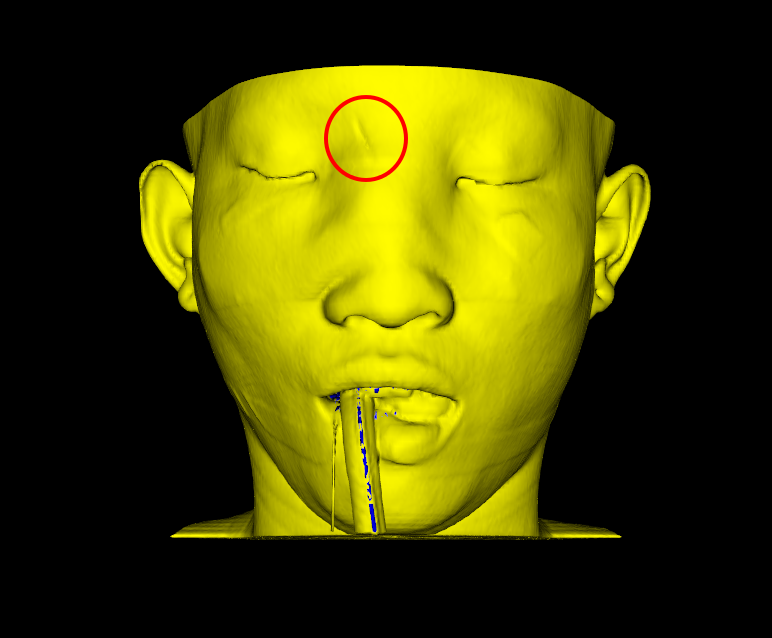
\includegraphics[width=\textwidth]{skull0}
			\caption{Frontal picture of the head. Notice the scar circled in
			red.}
			\label{fig:skull0}
	\end{subfigure}
	\quad
	\begin{subfigure}[b]{0.3\textwidth}
		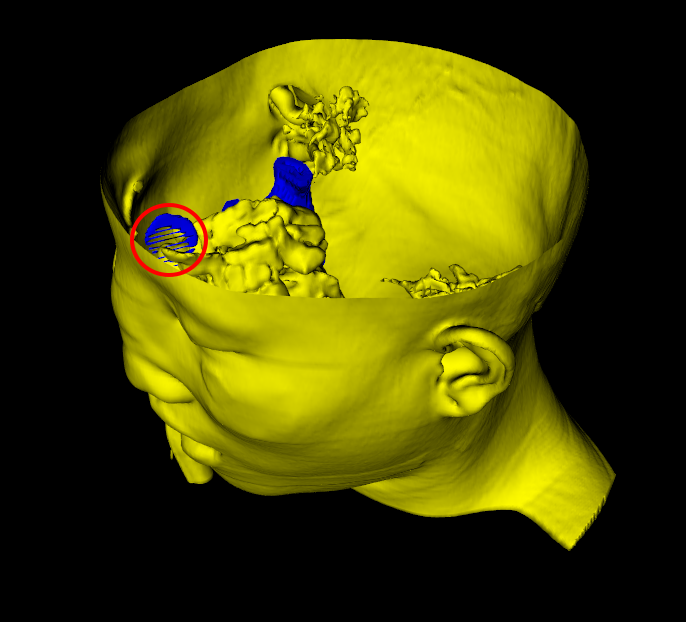
\includegraphics[width=\textwidth]{skull1}
			\caption{Foreign object lodged into head at scar position.}
			\label{fig:skull1}
	\end{subfigure}
	\quad
	\begin{subfigure}[b]{0.3\textwidth}
		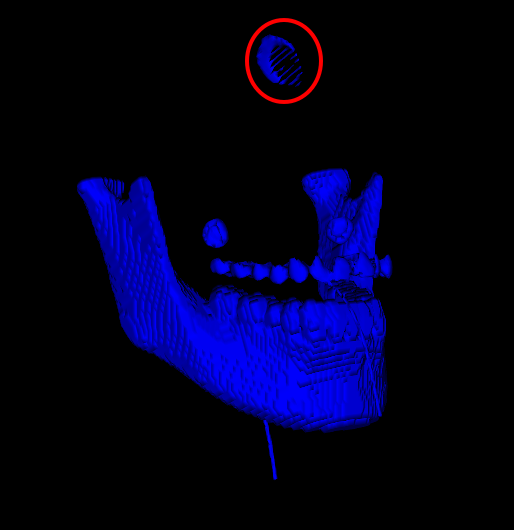
\includegraphics[width=\textwidth]{jaw}
			\caption{Jaw and foreign object only.}
			\label{fig:jaw}
	\end{subfigure}
	\caption{Skin displayed in yellow (isosurface of 700), dense bones and
	foreign object displayed in blue (isosurface of 3000)}\label{fig:skulls}
\end{figure}

\end{document}

